\Answer
Suppose we have a system of $N$ particles with number density $\rho$, thus the
box size will be

\begin{equation}
    L = \bigg( \frac{ N }{ \rho } \bigg)^{1 / 3}.
\end{equation}

If we want to impose the periodic boundary conditions (PBCs) here, we should adopt the
nearest image convention (NIC) or minimum image convention (MIC). What is an image? First,
we should emphasize that we could not do simulations in an infinitely large box (cell) in MD
simulations. The most common solution is to take one cell (we will call it ``center cell''
in the following text) to simulate and imagine an infinitive number of image cells
surrounding it, where each image cell is a replica of the center cell. The image cells can
reduce or eliminate boundary effects by providing every particle an equivalent surrounding
environment of particles as if it were in the bulk, no matter where they are in the center
cell.

\begin{figure}[h]
    \centering
    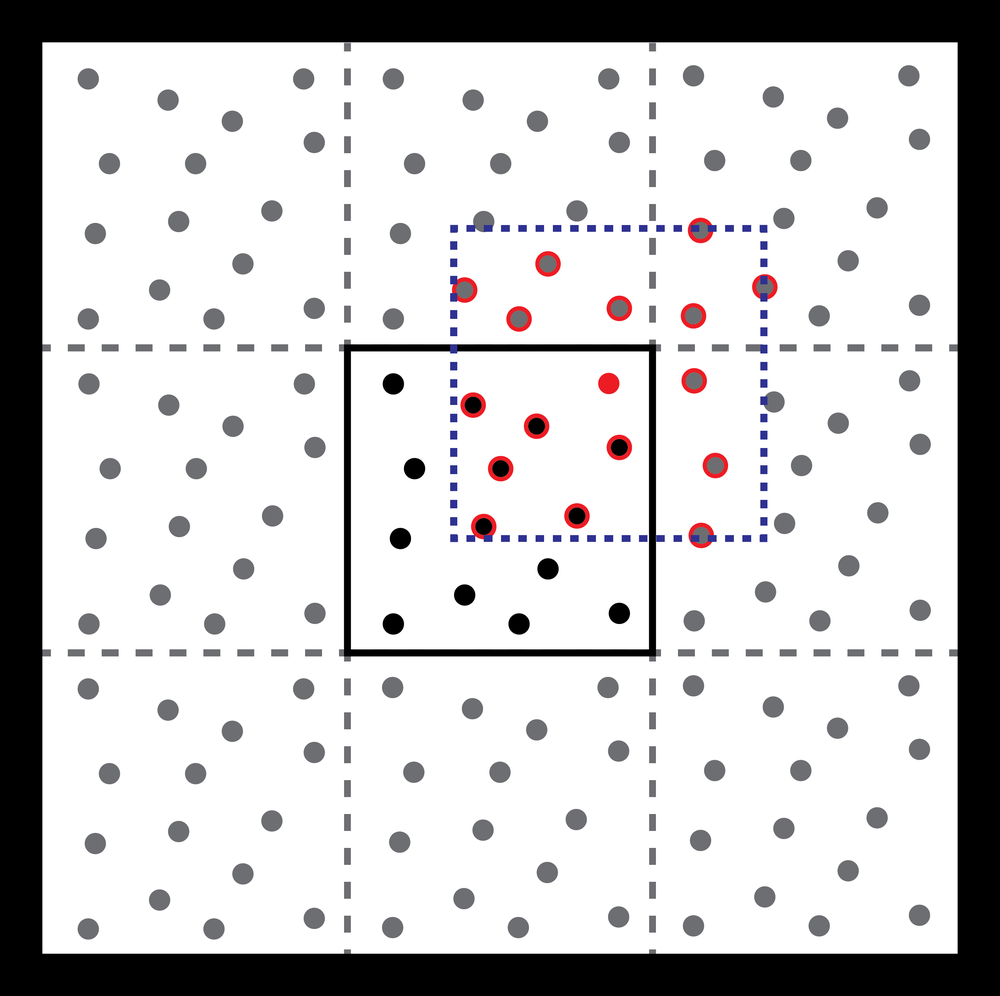
\includegraphics[width=0.5\textwidth]{nic}
    \caption{A center cell surrounded by $8$ more image cells with the same
        particles' relative locations and movements. Figure is from \cite{matlab}.}
    \label{fig:nic}
\end{figure}

When applying PBCs, particles near the edge of the cells often interact
with an image particle rather than a particle in the cell. For example, we can create the
situation shown below.
In Figure~\ref{fig:nic}, the black border box is our center cell, and the $8$ others are
its replica. The relative positions and velocities of the particles in these image cells
are exactly the same as their originals in the center cell. The red particle in the
upper left corner of the center cell only interacts with its neighbors: some of the
particles in the center cell plus some of the image particles in the image cells.
We call the box enclosing the red particle's neighbors a ``virtual image cell''.
The size of the virtual image cell (cutoff radius) is usually chosen as $L / 2$
of the center cell. That is, any particle which is more than $L / 2$ away from the
red particle in any direction is not included in the virtual image cell.
If the cutoff radius is larger than $L / 2$, it may lead to
unphysical self-interactions, sometimes called an artifact.

Another aspect of the PBCs is that when a particle hits a cell wall, instead of bouncing
back, it reappears on the other side of the cell (the topology of a torus), or we can
treat it as an image particle from an adjacent cell enters the current cell.
So the number of particles in a cell never increases or decreases in this case.

So how do we express the PBCs in mathematical and programming languages?
Suppose we have two particles, $a$ and $b$, both in the center cell,
and $a$ is the particle in which we
are interested. The vector pointing from $a$ to $b$ is the difference between
their positions:
%
\begin{equation}
    \bm{r} = \bm{r}_b - \bm{r}_a.
\end{equation}
%
For any component $r_\alpha$ of $\bm{r}$, where $\alpha = 1, 2, 3$, if its absolute value
is larger than $L / 2$, then we know $b$ is too far from $a$ to have effects on it,
so we should shift $b$ closer to $a$ in the corresponding dimension:
%
\begin{equation}
    \begin{cases}
        r_{b, \alpha} - L, & \text{if } r_\alpha > L / 2,                  \\
        r_{b, \alpha} + L, & \text{if } r_\alpha < -L / 2,                 \\
        r_{b, \alpha},     & \text{if } \lvert r_\alpha \rvert \leq L / 2,
    \end{cases}
\end{equation}
%
where $r_{b, \alpha}$ is the component of the position of particle $b$ in the
corresponding dimension.
The Julia code for the above procedure looks like Snippet~\ref{lst:nic}.
The code will return a \code{Vector} representing the new position of particle $b$.

\begin{algorithm}
    \caption{Find the nearest image of particle $b$ which can interact with particle $a$.}
    \label{lst:nic}
    \begin{juliacode}
        Δ𝐫 = b.position - a.position
        position = map(b.position, Δ𝐫) do rᵢ, Δrᵢ
            if Δrᵢ > L / 2
                rᵢ - L
            elseif Δrᵢ < -L / 2
                rᵢ + L
            else  # |Δrᵢ| <= L / 2
                rᵢ  # Do not shift
            end
        end
    \end{juliacode}
\end{algorithm}

If $b$ is not in the same cell as $a$, we need first shift $b$ back to the cell where
$a$ locates. That is,
%
\begin{equation}\label{eq:pbcs}
    (r_{b, \alpha} + 2L) \mod L,
\end{equation}
%
where adding $2L$ is to catch any runaway particles\cite{Adrian} with $r_{b, \alpha} < -L$.
The code representing \eqref{eq:pbcs} is in Snippet~\ref{lst:pbcs}.
%
\begin{algorithm}
    \caption{Move particle $b$ back to the center cell.}
    \label{lst:pbcs}
    \begin{juliacode}
        const L = 11.2  # Any real number you want
        f(rᵢ) = mod(rᵢ, L)
        b.position = map(f, b.position)
    \end{juliacode}
\end{algorithm}
%
Here Julia already provides the modulo function (it works for floating point numbers)
\href{https://docs.julialang.org/en/v1/base/math/#Base.mod}{\code{mod}}. Python and C++
also have similar functions. And since $L$ is always positive, we do not need to worry
about some nasty cases.
In the snippet, we \code{map} function \code{f} over
each component of the $b$'s position.

\begin{figure} % 2 subfigures
    \centering
    \begin{minipage}[t]{0.5\linewidth}
        \centering
        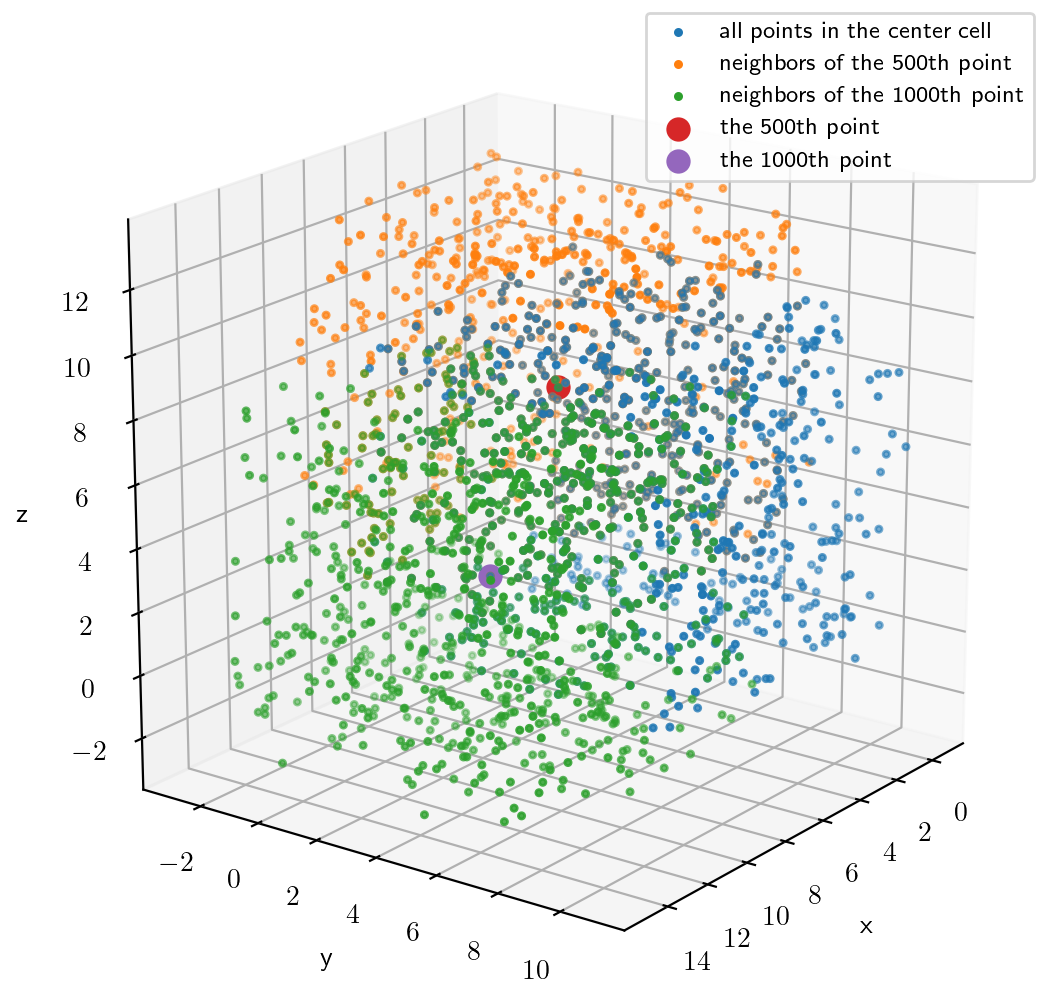
\includegraphics[width=\linewidth]{neighbors_profile}
        \subcaption{Viewing from one angle of neighbors of the selected particles.}
        \label{fig:neighbors:a}
    \end{minipage}
    \hfill
    \begin{minipage}[t]{0.5\linewidth}
        \centering
        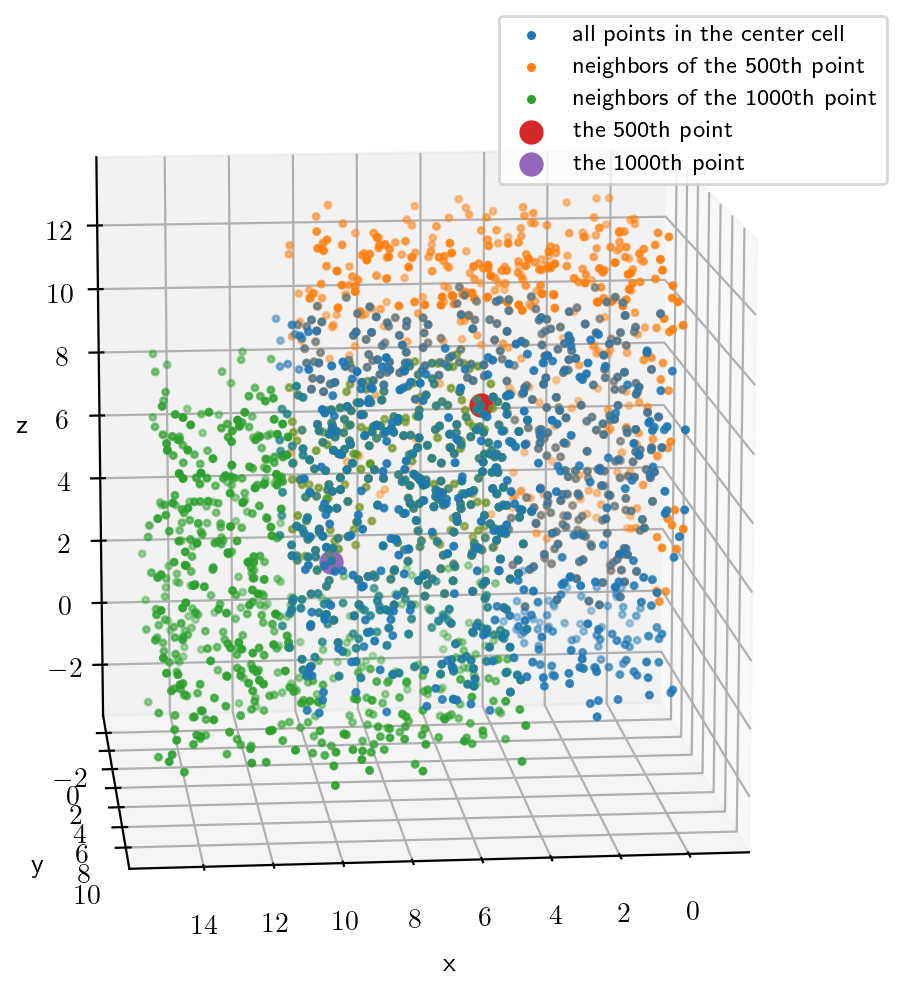
\includegraphics[width=\linewidth]{neighbors_front}
        \subcaption{Viewing from another angle of neighbors of the selected particles.}
        \label{fig:neighbors:b}
    \end{minipage}
    \caption{A system of $1000$ particles with $L \approx 11$. The blue points denote all
        the points in the center (original) cell, and the red and purple spheres are the
        $500$th and $1000$th particle among them. The orange and green points are the
        neighbors of these points which have interactions with them.}
    \label{fig:neighbors}
\end{figure}

To ensure that we have the correct neighbors, we need to plot the positions of these particles.
As shown in Figure \ref{fig:neighbors}, we have a system of $1000$ particles with
$\rho = 0.75$, so $L \approx 11$. The blue points denote all
the points in the center (original) cell, and the red and purple spheres are the
$500$th and $1000$th particles among them. The orange and green points are the
neighbors of these points which have interactions with them. That is, they are bounded by a
cubic whose centers are the $500$th and $1000$th particles,
with size $L \approx 11$ in each dimension.
There are $999$ points in both orange and green ``clouds'', and they do have overlaps
with the blue ``cloud''. From this, we know there is no double counting in our algorithm.

The syntax in Snippet \ref{lst:nic} and \ref{lst:pbcs} may confuse users as we
have not mentioned how we represent particles in
code. In our code, a \code{Particle} is simply a \code{mutable struct} wrapping two
\code{MVector}s (position and velocity), each with three \code{Float64} values, as shown in
Snippet~\ref{lst:particle}. So \code{b.position} (\code{b.velocity}) is how we access the
stored data of its position (velocity).

\begin{algorithm}
    \caption{The definition of a particle in our code.}
    \label{lst:particle}
    \begin{juliacode}
        using StaticArrays: MVector

        mutable struct Particle
            position::MVector{3,Float64}
            velocity::MVector{3,Float64}
        end
    \end{juliacode}
\end{algorithm}

Now let us talk about the Lennard--Jones potential.
The original form of the two-particle potential would look like~\eqref{eq:uljunit}:
%
\begin{equation}\label{eq:uljunit}
    u(r_{ij}) = 4 \varepsilon \biggl( \Bigl( \frac{ \sigma }{ r_{ij} } \Bigr)^{12}
    -\Bigl( \frac{ \sigma }{ r_{ij} } \Bigr)^6 \biggr),
\end{equation}
%
where the parameters for \ce{Ar} are $\varepsilon = \SI{0.0104}{\electronvolt}$,
$\sigma = \SI{3.40}{\angstrom}$, and $m = \SI{39.948}{\atomicmassunit}$, where
$\si{\atomicmassunit}$ is the atomic mass unit.
In the dimensionless form,
\eqref{eq:uljunit} would look like~\eqref{eq:ulj} and the force would
look like~\eqref{eq:flj}.
%
\begin{align}
    u(r_{ij})                      & = 4 \biggl( \Bigl( \frac{ 1 }{ r_{ij} } \Bigr)^{12}
    -\Bigl( \frac{ 1 }{ r_{ij} } \Bigr)^6 \biggr), \label{eq:ulj}                        \\
    \frac{ d^2 \bm{r}_i }{ d t^2 } & = 48\sum_{j \neq i} (\bm{r}_i - \bm{r}_j)
    \biggl( \Bigl( \frac{ 1 }{ r_{ij} } \Bigr)^{14}
    -\frac{ 1 }{ 2 } \Bigl( \frac{ 1 }{ r_{ij} } \Bigr)^8 \biggr). \label{eq:flj}
\end{align}
%
And the numerical gradient of~\eqref{eq:ulj} is
%
\begin{equation}\label{eq:dudr}
    \begin{bmatrix}
        \nicefrac{ \partial u }{ \partial x } \\
        \nicefrac{ \partial u }{ \partial y } \\
        \nicefrac{ \partial u }{ \partial z }
    \end{bmatrix}
    \Rightarrow
    \begin{bmatrix}
        \nicefrac{ \big( u(\bm{r} + dx \hat{\bm{x}}) - u(\bm{r}) \big) }{ dx } \\
        \nicefrac{ \big( u(\bm{r} + dy \hat{\bm{y}}) - u(\bm{r}) \big) }{ dy } \\
        \nicefrac{ \big( u(\bm{r} + dz \hat{\bm{z}}) - u(\bm{r}) \big) }{ dz }
    \end{bmatrix}.
\end{equation}
%
I found in the notes, equation \eqref{eq:flj} is off by a factor of $48$.
Only after adding it could make \eqref{eq:dudr} and \eqref{eq:flj} match.
I suppose that this is because we basically treat
$\varepsilon$, $\sigma$, and $m$ (the mass of each particle) as $1$ here (though they
are not). So in Snippet~\ref{lst:gradient} I define the $\nabla u$ and the acceleration
particle $a$ experiences (induced only by particle $b$) as below.
%
\begin{algorithm}
    \caption{The gradient of the Lennard--Jones potential and the acceleration
        $d^2 \bm{r}_a / d t^2$. Note the factor $48$ and the negative sign.}
    \label{lst:gradient}
    \begin{juliacode}
        function potential_gradient(𝐫ᵢⱼ)
            rᵢⱼ = norm(𝐫ᵢⱼ)
            return 48𝐫ᵢⱼ * (inv(rᵢⱼ^8) / 2 - inv(rᵢⱼ^14))
        end

        function Acceleration(a::Particle)
            return function (b::Particle)
                return Acceleration(-potential_gradient(a.position - b.position))
            end
        end
    \end{juliacode}
\end{algorithm}
%
The negative sign indicates the force is the negative gradient of the potential.
To get the total potential energy of the swarm of particles, we sum up all the $i$'s
and $j$'s (except for $j = i$) in~\eqref{eq:uij}:
%
\begin{equation}\label{eq:U}
    U = \frac{ 1 }{ 2 }\sum_{\substack{i, j\\ j \neq i}} u(r_{ij}).
\end{equation}
%
Note the $\frac{ 1 }{ 2 }$ factor in \eqref{eq:U} since we count $i$ and $j$ twice.
Snippet \ref{lst:U} does the same thing:

\begin{algorithm}
    \caption{Calculate the total Lennard--Jones potential energy of a swarm of particles.}
    \label{lst:U}
    \begin{juliacode}
        function potential_energy(particles::Vector{Particle})
            return 1 / 2 * sum(eachindex(particles)) do i
                sum(filter(!=(i), eachindex(particles))) do j
                    potential_energy(particles[i], particles[j])
                end
            end
        end
    \end{juliacode}
\end{algorithm}

Similarly, we need to calculate the total force (acceleration) of all the other particles
enforced on one particle, as shown in \eqref{eq:flj}. Now we need to employ the
\code{list_neighbors} function we used to calculate one particle's neighbors and plotted
Figure \ref{fig:neighbors}, as shown in \ref{lst:flj}.
%
\begin{algorithm}
    \caption{Calculate the total Lennard--Jones force a particle experiences.}
    \label{lst:flj}
    \begin{juliacode}
        function acceleration(cell::Cell, particle::Particle)
            neighbors = list_neighbors(cell, particle)
            return sum(Acceleration(particle), neighbors)
        end
    \end{juliacode}
\end{algorithm}
%

